\section{Global Correlation}
\label{sec:2}
In this section, I introduce the term \textit{global correlation}, the base \textit{naive} approach, explain \textit{iBRAID} algorithm, which uses an efficient principle of calculating the correlation coefficient, and show \textit{PriCe} for interactive pairwise correlation of subsequences of time-series data.
\subsection{Foundations}
Correlation may occur in a burst, last for a certain duration, and then disappear. Without loss of generality, the data streams are running synchronously and sampled at a fixed rate, data are numeric, and all time-series are of the same length so that they can be treated as discrete signal sequences. It means that the two data streams are aligned with each other in the time dimension, and there are no missing timestamps. To simplify the problem and the algorithm's explanations, it will discuss only how to detect a correlation between two data streams, but then it is possible to extend the detection to multiple time-series data streams. To continuously detect the correlation of two streams, a sliding window is applied to keep the most recent synchronous subsequences of the streams.~\cite{ref2} \newline

The numerical time-series data streams are denoted as $X$ and $Y$, so $x = \{x(0), \\x(1),\ldots,x(N- 1)\}$ stands for the subsequence of $X$ with limited length $N$, where $x(n) \in \mathbb{R}$ is the value of the $(n + 1)$-th data point of the subsequence. $len(x)$ is the length of $x$, and $st(x)$ is the starting time unit of $x$. Similar concepts are also applied to $Y$. Here, the correlation is evaluated by the widely applied Pearson correlation coefficient. For two sequences $X$ and $Y$, which have the same length $N$ and the same starting time unit, the Pearson correlation coefficient is calculated as, where $\bar{x}$ and $\bar{y}$ stand for the mean value of $x$ and $y$ respectively:
\begin{equation}
\label{equ:1}
r_{x y}=\frac{\sum_{n=0}^{N-1}\left(x_{n}-\bar{x}\right)\left(y_{n}-\bar{y}\right)}{\sqrt{\sum_{n=0}^{N-1}\left(x_{n}-\bar{x}\right)^{2}} \sqrt{\sum_{n=0}^{N-1}\left(y_{n}-\bar{y}\right)^{2}}}
\end{equation}
The term $r_{x y} \in[-1,1]$ indicates the linear correlation of the sequences and can reflect the similar behavior of sequence trend. Theoretically, when the evaluated parts of two sequences are correlated, $r_{x y}$ will return a value close to $\mbox{1 or -1}$.

\subsection{Naive Solution}
The naive solution is the most apparent approach to finding and reporting correlated subsequences in a time-series data set. First, the approach starts with a single pair of time series, picks subsequences of them, which start at the same point in time, and calculates the Pearson correlation coefficient for them. Subsequently, it continues the Pearson correlation coefficient calculations for other subsequences of the same pair of time-series, or moves to calculate the Pearson correlation coefficient for the corresponding subsequences of different pairs of time-series until all possible pairs of subsequences in the time-series data set are examined. Finally, it returns all pairs of subsequences whose Pearson correlation coefficient meets a threshold. As a result, each pair decides correlation.\newline 

There is an advantage that it is pretty easy to implement, but also a disadvantage that there is a complex calculation using the central math equation \hyperref[equ:1]{(1)} for all pairs of time-series in the data set. In other words, the naive approach illustrates the crux of the problem, which is the high number of calculations required to explore the data sets. This algorithm does not have any prior knowledge about the data and does not use any results as a decision-making input to speed up the production of results. Additionally, each point in each time series is touched as many times as the different pairs of time-series in the data set are.

\subsection{iBRAID Solution~\cite{ref2,ref3}}
\label{sec:iBRAID}
\begin{figure}[H]
\centering
    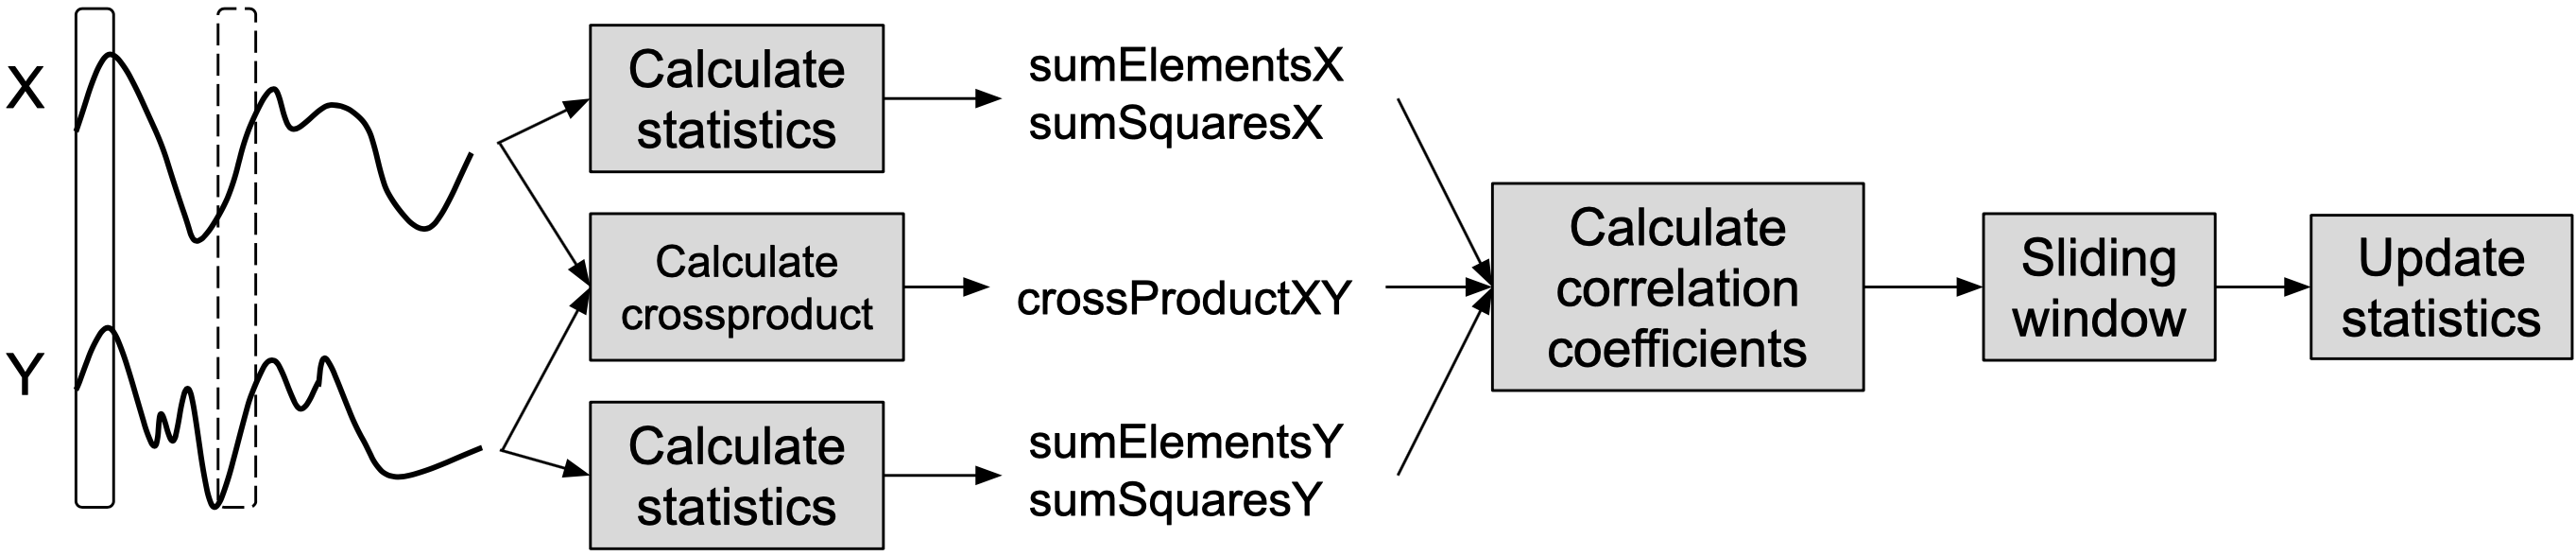
\includegraphics[width=\textwidth]{figures/ibraid.png}
    \caption{The iBRAID approach.}
    \label{fig:iBRAID}
\end{figure}
The iBRAID algorithm originated from the work BRAID, described in 2005.~\cite{ref6} This solution is based on the hypothesis that integrating caching can achieve interactivity. The iBRAID technique partially solved the problem of the naive approach by efficiently calculating the Pearson correlation coefficient based on basic and computationally cheap five sufficient statistics — the sum of the data points in each window of length $m$ ($s u m_{x}$), the sum of the squares of the data points of each window of length $m$ ($s u m_{x x}$), the inner cross-product of the data points of the two windows of length $m$ ($s u m p r o d_{x y}$), the variance for time-series ($v a r_{x}$), and the covariance of the two time-series ($c o v_{x y}$) for which the correlation is calculated. The covariance of the two time-series $X$ and $Y$ is
\begin{equation}
c o v_{x y}=s u m p r o d_{x y}-\frac{s u m_{x} \times s u m_{y}}{m}
\end{equation}
and the variance of the window of length $m$ can be calculated according to the following equation
\begin{equation}
v a r_{x}=s u m_{x x}-\frac{(s u m_{x})^{2}}{m}
\end{equation}
Similarly, the variance for time-series $Y$ will be denoted $v a r_{y}$. Then, the Pearson correlation coefficient can be calculated by applying the following equation
\begin{equation}
r_{x y}=\frac{c o v_{x y}}{\sqrt{v a r_{x} \times v a r_{y}}}
\end{equation}
First, the approach analyzes the pairs of data streams sequentially, starting from the first point for all data streams. It calculates the sufficient statistics needed to calculate the Pearson correlation coefficient efficiently. Next, it calculates the Pearson correlation coefficient for the first point for all pairs of windows. Once this is done, the windows are slid further by one point, and the sufficient statistics are updated incrementally — the first point is expired/subtracted from them, and the new point is added. The Pearson correlation coefficient is calculated again for all pairs. Then, it analyzes all data streams by a single point, augmenting the sufficient statistics incrementally and recalculating the Pearson correlation coefficient. This is done until the whole pair is analyzed.\newline

Now, I focus on the idea of an incremental approach. These sufficient statistics can be computed either from scratch or incrementally each time a new point of data streams explores a pair of data streams. In this case, the sums stored in memory are incremented by the new values and decremented by those not part of the windows anymore. The same operations are performed for the sums of the squares and the inner cross products using the respective points of data streams. So, iBRAID is a round-robin scanning algorithm that uses the incremental computation of the Pearson correlation coefficient. \newline

Method iBRAID has the following advantages: it is easy to implement, it reduces the computations by half due to the usage of sufficient statistics, and it uses an incremental approach. iBRAID is experimentally shown to perform well for data streams whose data is uniformly distributed and for low correlation thresholds. On the other hand, it might underperform on skewed data sets.

\subsubsection{Evaluation}
The authors have used Yahoo Finance Historical Data Set\footnote{Yahoo Inc. Yahoo Finance Historical Data (2016). \href{https://finance.yahoo.com/quote/YHOO/history}{https://finance.yahoo.com/quote/YHOO/history}}: It consists of 318 time series and reflects the trading of 56 companies on the New York Stock Exchange for the last 28 years. The length of each time series is about 7100 timestamps. \newline

Naive and iBRAID have the same number of operations due to exhaustive processing of the pairs. The authors noticed that the higher the Pearson correlation coefficient, the more operations the algorithm executes. This is due to fewer windows that are highly correlated according to the Pearson correlation coefficient. This results in higher latency in detecting them by the algorithm. On the other hand, in the case of a low Pearson correlation coefficient, the authors saw that iBRAID terminates the analysis process early, as soon as it reaches the criterion of the number of correlated sliding windows. 

\subsection{PriCe Solution~\cite{ref1,ref4}}
\begin{figure}[ht]
\centering
    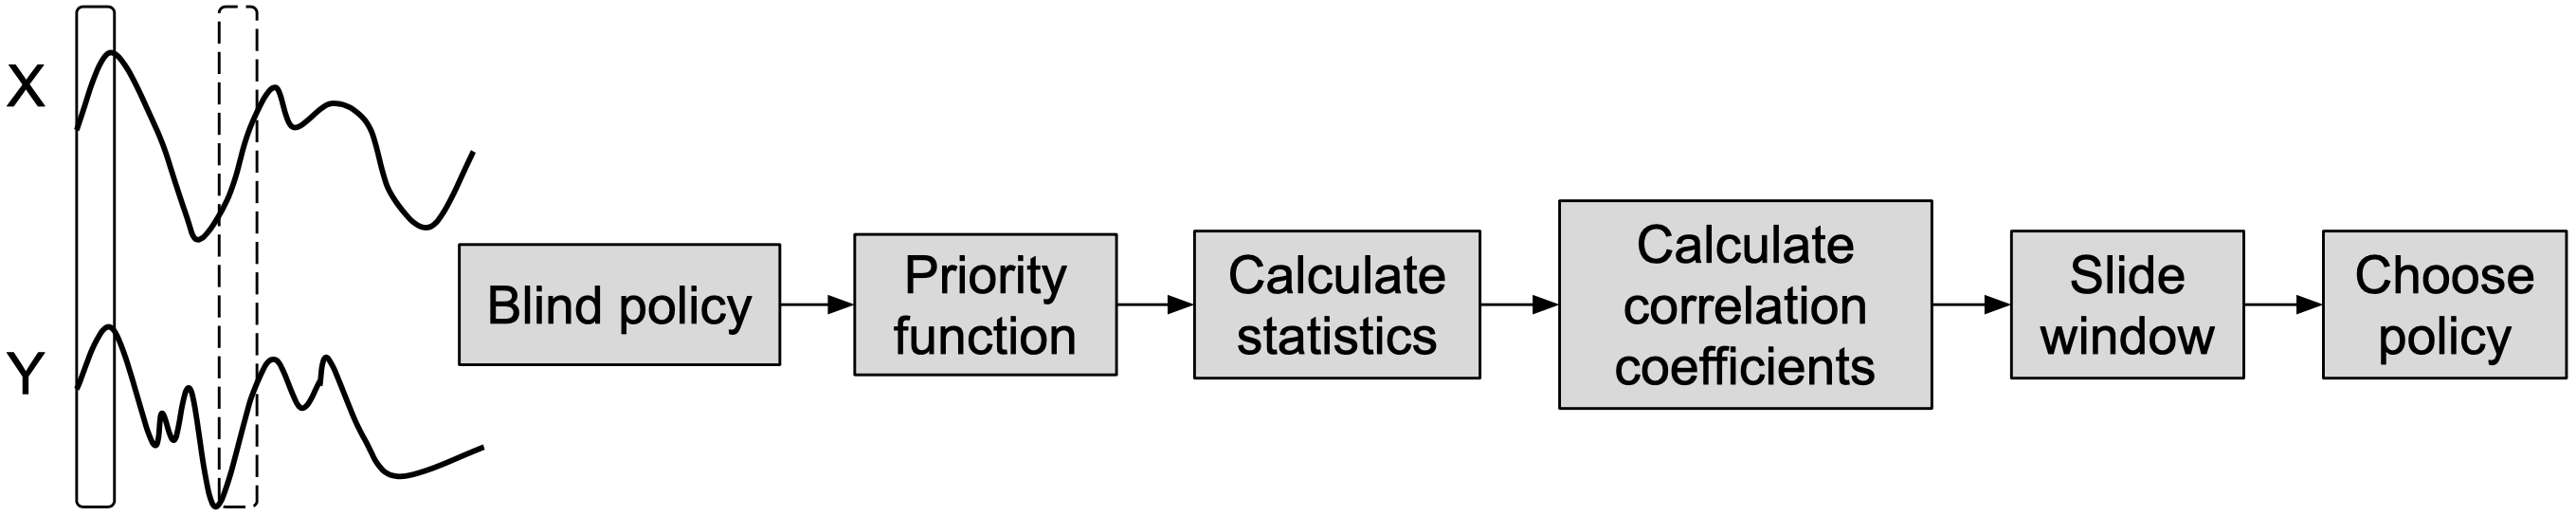
\includegraphics[width=\textwidth]{figures/price.png}
    \caption{The PriCe approach.}
    \label{fig:PriCe}
\end{figure}
PriCe is a more informed search algorithm. It uses a priority function to explore the pairs of subsequences while reusing partial Pearson correlation coefficient computations as the iBRAID approach. This solution is based on the hypothesis that interactivity can be achieved by integrating caching and scheduling principles. The idea of PriCe is to explore the most promising pair first, the one with the highest priority function value. The priority function:
\begin{equation}
P r=P C C *(M / t o t a l E x p) / C
\end{equation}
where \textit{PCC} is the most recently calculated Pearson correlation coefficient for a pair of sliding windows that belong to the same pair of data streams, \textit{M} is the number of correlated sliding windows found in the corresponding pair of data streams so far, \textit{totalExp} is the total number of analyzed pairs of sliding windows, and \textit{C} is the cost of analyzing a pair of sliding windows in terms of number of computations. The default values are \textit{PCC} = 1, \textit{M} = 0, $\mbox{\textit{totalExp} = 1}$, and $\mbox{\textit{C} = 1}$.\newline

PriCe prioritizes the pair of time series with a history of increased results produced so far and a highly recently calculated Pearson correlation coefficient. This captures the idea of space locality along with temporal locality, where the recently estimated Pearson correlation coefficient captures space locality, and the ratio of correlated sliding windows captures temporal locality to the total number of analyzed pairs of sliding windows. Moreover, the cost in the priority function is the number of operations needed to calculate the sufficient statistics for a pair of sliding windows. For example, if a pair of data streams share one data stream with another pair. Then, the more advanced one (i.e., the one with a higher timestamp in the interval) has already calculated the sums and the sum of the squares for the tuples of that data stream. This leaves the lagging behind pair with lower cost to slide its windows since the more advanced one has already computed some of the sufficient statistics for that shared data stream.\newline

The authors of this approach implemented and evaluated nine policies that initialize and/or tune the priority function. It is based on the concepts of early termination and pruning. When the first pair arrives at the system, the system does not know any correlated pairs of streams.
\begin{enumerate}
\item \textit{Blind}: when the analysis starts with no prior knowledge of correlated pairs of streams, Blind policy initializes PriCe's priority function to its default values.
\item \textit{Informed}: the priority function is initialized based on the latest analysis results. In the Informed starting phase, PriCe’s priority function is initialized to the same parameter values of the correlated pairs used by the immediately previous subsequences. The rationale behind this policy is to keep analyzing closely those pairs that already exhibited a high correlation in the earlier subsequences, potentially indicating an insight of interest.
\item \textit{Untouched}: the focus is on the pairs not processed in the previous iterations (i.e., not chosen for analysis due to their low values of Pearson correlation coefficient) at the beginning of PriCe's execution. Specifically, such pairs are jumpstarted by altering their previous number of correlated windows. This increases their priority, preventing starvation and giving them another chance to be analyzed in the new iteration. The rationale behind this policy is to allow such pairs another chance, potentially identifying different behaviors that remained undetected in the previous iteration.
\item \textit{Alternating}: this policy gives the pairs that were not correlated in the previous iteration a chance to be explored through a hybrid round-robin fashion. In the Alternating starting phase, alternately, a pair from those that are not correlated in the previous iteration is picked and explored using PriCe, followed by a pair from those that were correlated. By doing this, the idea is to reduce starvation's effect for those not correlated in the previous iteration.
\item \textit{X\% Non-correlated}: this policy tries to achieve fairness of exploration through jumpstarting the lowest X\% pairs in priority. The pair with the highest priority among those lowest X\% is picked and explored. This continues until all those X\% pairs are jumpstarted. Consecutively, PriCe carries out the exploration process naturally.
\item \textit{Decaying History}: this policy regards the significance of the whole historical correlation information of a pair differently from recent iterations information. In the priority function, it alters the parameter \textit{M}, which reflects the number of correlated sliding windows found for a corresponding pair, such that it becomes weighted. It gives the historical correlation information a weight and then a higher weight to the most recent correlation information. Then, the total of both becomes the new parameter \textit{M}. This policy aims to consider the most recent information along the exploration process instead of older ones.
\item \textit{Shared Stream}: Its focus is on the group of pairs not correlated in the previous iteration but sharing a data stream that was part of a correlated one in the preceding iteration. The idea in this policy is that a data stream that is correlated with another one might also be correlated with a third different stream. Thus, this policy picks a pair from this group of non-correlated pairs according to PriCe and explores it. Shared Streams starts all those pairs and then carries on using PriCe.
\item \textit{X\% Probing}: this policy explores the first few windows for all the pairs in a round-robin fashion. This is done to set the priority function with actual current values instead of artificial hand-crafted ones. After those few windows, PriCe kicks in and continues the exploration process using the priority function with its parameters filled with actual data through the probing process.
\item \textit{P-Alternating}: this policy mimics the multilevel queue scheduling, whereby the pairs are explored in a round-robin fashion between two groups. Those are the previously correlated pairs and the non-correlated ones. This gives the pairs not correlated in the previous iteration a chance to be persistently processed. It picks a pair from the non-correlated ones and processes it using PriCe; then, it picks a pair from those correlated. It does that until the end of the iteration and carries on in this fashion by selecting the pair from each group of pairs according to the priority function. By doing this, the hope is to alleviate the effect of starvation for those pairs that were not persistently correlated in the previous iteration, for they might exhibit some correlation beyond the starting phase.
\end{enumerate}

\subsubsection{Evaluation}
The authors have used the same data set from Yahoo (as described in Sect.\hyperref[sec:iBRAID]{2.3}). Naive and PriCe have the same number of operations due to the exhaustive processing of the pairs. The authors noticed that the higher the Pearson correlation coefficient, the more operations the algorithm executes. This is due to fewer windows that are highly correlated according to the Pearson correlation coefficient. On the other hand, in the case of a low Pearson correlation coefficient, the authors saw that terminates the analysis process early.\newline

The authors noticed that PriCe outperformed the naive algorithm and the iBRAID approach in experiments. This is a speed-up of more than 15 times than the iBRAID solution. This is attributed to the pruning and early termination features, which allow the algorithm to analyze other pairs and detect more correlated data streams. The authors saw that PriCe scheduling demonstrated the effectiveness of its priority function in capturing more correlated pairs at an early deadline, especially when the Pearson correlation coefficient is high. That means it elects the pairs to explore more intelligently than the naive and iBRAID approaches.\newline

The authors noticed that PriCe with policy \textit{P-Alternating} is the best policy for detecting correlated live data streams for high values of the Pearson correlation coefficient. On the other hand, the \textit{1\% Probing} outperforms the rest when the Pearson correlation coefficient has low values. This is attributed to the fact that with higher Pearson correlation coefficient values, it is highly likely to have fewer correlated windows in a given pair and vice versa. Finally, the explorative policies (i.e., \textit{Blind}) achieved the highest diversity in detecting new correlated pairs than the exploitative ones (i.e., \textit{Informed}, \textit{Untouched}, and \textit{P-Alternating}). This can be explained because the exploitative policies have some informative approach to analyzing the data streams, whether from previous iterations or some other source. Thus, they will keep exploring the pairs already correlated in previous iterations.